\chapter{Organizzazione dei protocolli in livelli}

Un termine che si utilizza frequentemente quando si parla di Internet è protocollo.
\begin{redbar}
    Un \textbf{protocollo} definisce le regole che il mittente e il destinatario, così come tutti i sistemi intermedi coinvolti, devono rispettare per essere in grado di comunicare.
\end{redbar}

In situazioni particolarmente semplici potrebbe essere sufficiente un solo protocollo, in situazioni più complesse potrebbe essere opportuno suddividere i compiti fra più livelli (layer), nel qual caso è richiesto un protocollo per ciascun livello: si parla dunque di layering di protocolli, o di organizzazione (o strutturazione) dei protocolli in livelli.

\section{Due scenari}
\begin{Example}{Esempio di comunicazione}{}
    \textit{In questo esempio si sviluppano due scenari per comprendere meglio la necessità di organizzare i protocolli in livelli:}
    \begin{enumerate}
        \item Si ipotizzi che Maria e Anna siano vicine di casa con molti interessi in comune. La comunicazione fra di loro avviene direttamente con un solo livello, faccia a faccia e nella stessa lingua.

        Anche in questo semplice scenario è comunque necessario rispettare un certo insieme di regole. Per prima cosa Anna e Maria sanno che è buona norma salutarsi appena si incontrano. Secondo, sono coscienti di poter utilizzare uno stile di linguaggio adatto al loro livello di confidenza. Terzo, riconoscono di doversi astenere dal parlare mentre la controparte sta parlando. Quarto, sono coscienti che la conversazione dovrebbe essere un dialogo piuttosto che un monologo: entrambe le parti devono avere la possibilità di esprimersi. Quinto, sanno che è opportuno scambiare qualche convenevole prima di lasciarsi.

        \begin{minipage}{\textwidth}
            \centering
            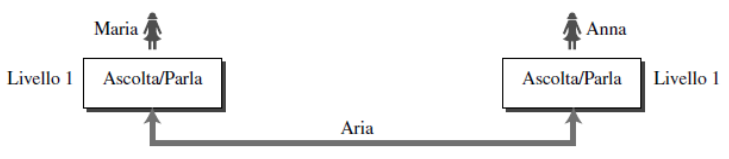
\includegraphics[width=0.7\linewidth]{images/anna-maria1.PNG}
            %\captionof{figure}{Esempio}
        \end{minipage}

        \item Si ipotizzi che ad Anna venga offerta una posizione migliore nella azienda in cui lavora, e che debba traslocare in altra sede in una città molto lontana da Maria. Le due amiche decidono dunque di continuare le loro conversazioni utilizzando il servizio postale, ma senza rischiare che altre persone possano venire a conoscenza delle loro idee se le loro lettere venissero intercettate. Di conseguenza si accordano per crittografare i messaggi: il mittente di una lettera la cripta per renderla incomprensibile a un eventuale intruso, il destinatario della lettera la decripta per recuperare il messaggio originale. In questo caso la comunicazione fra Anna e Maria avviene su tre livelli. Si ipotizza che le due amiche abbiano tre macchine ciascuna, per portare a termine i compiti a ciascun livello.

        Si ipotizzi ora che Maria invii la prima lettera ad Anna: comunica quindi con la macchina al terzo livello. La macchina di terzo livello ascolta quanto dice Maria e crea il testo in chiaro, che viene passata alla macchina del secondo livello. Questa riceve il testo in chiaro, lo cripta e ottiene il testo cifrato che viene passato alla macchina del primo livello. Quest'ultima, prende il testo cifrato, lo mette in una busta, aggiunge gli indirizzi del mittente e del destinatario e la invia.

        Dal lato di Anna la macchina al primo livello recupera la busta dalla cassetta delle lettere, toglie quindi il testo cifrato dalla busta e lo consegna alla macchina di secondo livello. Questa decripta il messaggio ottenendo il testo in chiaro che passa alla macchina di terzo livello. Quest'ultima prende il testo in chiaro e lo legge.

        \begin{minipage}{\textwidth}
            \centering
            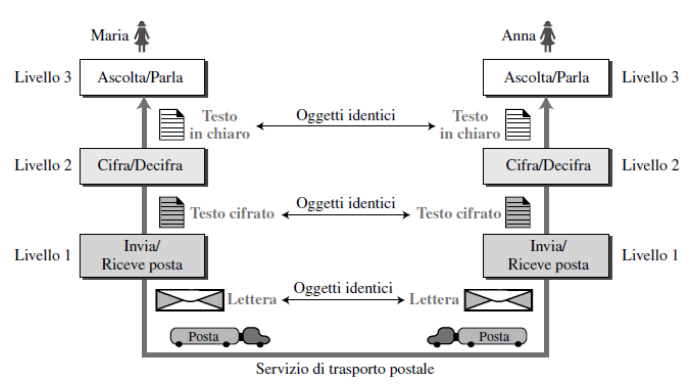
\includegraphics[width=0.7\linewidth]{images/anna-maria2.PNG}
            %\captionof{figure}{Esempio}
        \end{minipage}
    \end{enumerate}
\end{Example}

La strutturazione in livelli dei protocolli consente di suddividere un compito complesso in compiti più semplici. Nel esempio si sarebbe potuto utilizzare una sola macchina per portare a termine il compito delle tre macchine. Tuttavia se Maria e Anna decidessero che la tecnica crittografica utilizzata dalla seconda macchina non fosse più adeguata per proteggere i loro segreti, dovrebbero sostituire l'intera macchina. Nella situazione descritta, invece, è sufficiente sostituire solamente la macchina di secondo livello, lasciando inalterate le altre due. Questa tecnica viene chiamata modularizzazione, che in questo caso significa sostanzialmente indipendenza dei livelli. Un modulo, o meglio un livello in questo contesto, può essere descritto come una black box con opportuni ingressi e uscite, senza doversi preoccupare della modalità con la quale i dati in ingresso vengano trasformati nei dati di uscita. Se due macchine forniscono lo stesso output dato il medesimo input, possono essere considerate equivalenti. Per esempio Anna e Maria potrebbero acquistare la macchina di secondo livello da due produttori differenti, purché entrambe le macchine producano il medesimo testo cifrato dal medesimo testo in chiaro e viceversa.

Uno dei vantaggi della strutturazione in livelli è la possibilità di separare i servizi offerti e la loro implementazione. Un livello deve essere in grado di utilizzare un insieme di servizi dal livello inferiore per offrire servizi al livello superiore, indipendentemente da come sia implementato. Per esempio Maria potrebbe decidere di non comprare la macchina del primo livello ed effettuare i compiti richiesti personalmente.

Un altro vantaggio della strutturazione in livelli, che non si evidenzia in questi semplici esempi ma che diverrà evidente quando si discuterà l'organizzazione in livelli di Internet, è che la comunicazione non coinvolge necessariamente sempre solo due sistemi terminali: spesso vengono infatti coinvolti dei sistemi intermedi (per esempio, router) che richiedono solo alcuni livelli. Se non si utilizzasse il layering i sistemi intermedi dovrebbero avere la medesima complessità dei sistemi terminali, cosa che renderebbe il sistema più costoso.

\subsection{Principi della strutturazione in livelli}

In questo paragrafo si presentano alcuni principi fondamentali relativi alla strutturazione in livelli. Innanzitutto, quando è richiesta una comunicazione bidirezionale, è necessario rendere ciascun livello capace di effettuare i due compiti opposti, uno per ciascuna direzione. Per esempio il compito del terzo livello è ascoltare (in una direzione) e parlare (nell'altra direzione), il secondo livello deve essere in grado di crittografare e decrittografare, il primo livello deve poter inviare e ricevere la posta.

Il secondo principio da seguire riguarda gli oggetti in input/output sotto ciascun livello di entrambi i lati: devono essere identici. Per esempio l'oggetto sotto al livello 3 di entrambi i lati deve essere una lettera in chiaro, l'oggetto sotto al livello 2 deve essere una lettera cifrata. L'oggetto sotto al livello 1 di entrambi i lati deve essere una busta.

\subsection{Collegamenti logici}
Se si rispettano i due principi precedenti è possibile immaginare un collegamento logico fra i livelli, come mostrato nella Figura \ref{fig:collegamento-logico-livelli}.
Questo collegamento logico (virtuale) è come se consentisse una comunicazione diretta fra i pari livelli delle due parti.

\begin{figure}[ht]
    \centering
    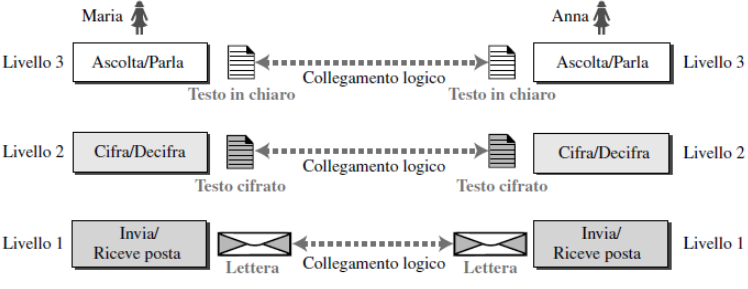
\includegraphics[width=10cm]{images/collegamento-logico-livelli.PNG}
    \caption{Collegamento logico tra i livelli}
    \label{fig:collegamento-logico-livelli}
\end{figure}

\section{Lo stack protocollare TCP/IP}
Chiariti i concetti di layering e di collegamento logico fra i livelli, è possibile introdurre l'architettura TCP/IP, ovvero la strutturazione in livelli dei protocolli utilizzati in Internet. Si tratta di una gerarchia di protocolli costituita da moduli interagenti, ciascuno dei quali fornisce funzionalità specifiche. Il termine gerarchia significa che ciascun protocollo di livello superiore è supportato dai servizi forniti dai protocolli di livello inferiore. Tale organizzazione dei protocolli viene chiamata pila o stack protocollare TCP/IP. Definita in origine in termini di quattro livelli software soprastanti a un livello hardware, la pila TCP/IP è oggi intesa come composta di cinque livelli.

\begin{figure}[ht]
    \centering
    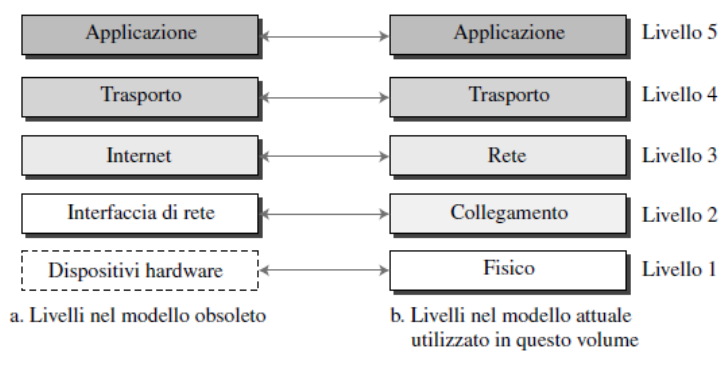
\includegraphics[width=10cm]{images/livelli-tcp-ip.PNG}
    \caption{Livelli nello stack protocollare TCP/IP}
    \label{fig:livelli-tcp-ip}
\end{figure}

\subsection{Architettura a livelli}

\begin{Example}{Comunicazione in una internet}{}
    \textit{Con l'obiettivo di illustrare come i vari livelli dello stack protocollare TCP/IP siano coinvolti nella comunicazione fra due host, si ipotizza che si vogliano utilizzare i protocolli TCP/IP in una piccola internet costituita da tre (link) LAN, ciascuna con uno switch di collegamento (data-link), interconnesse tramite un router.}

    \begin{minipage}{\textwidth}
        \centering
        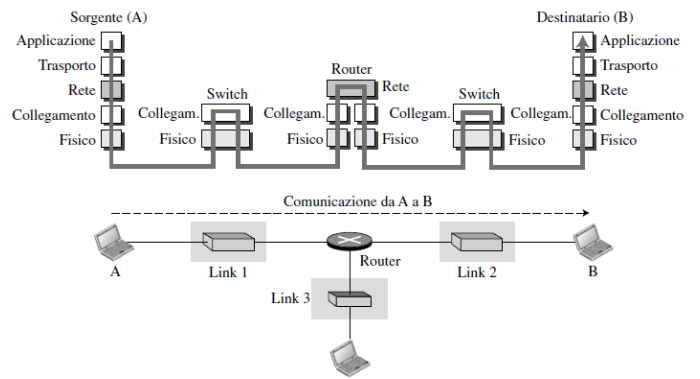
\includegraphics[width=0.8\linewidth]{images/comunicazione-livelli.PNG}
        %\captionof{figure}{Esempio}
    \end{minipage}

    Si supponga che l'host A comunichi con l'host B. L'host sorgente crea un messaggio a livello applicazione e lo trasmette attraversando verso il basso tutti e cinque i livelli in modo tale che possa essere fisicamente inviato all'host destinatario. Questo riceve il messaggio al livello fisico e lo consegna attraverso gli altri livelli all'applicazione destinataria.

    Il router è coinvolto solamente per tre livelli: i livelli trasporto e applicazione non hanno ragione di esistere in un router che venga utilizzato esclusivamente per scopi di instradamento. Sebbene un router abbia sempre un livello rete, può utilizzare $n$ combinazioni di livelli fisici e collegamento dove $n$ è il numero di link ai quali è collegato. Infatti ciascun collegamento potrebbe utilizzare un proprio specifico protocollo di livello fisico o collegamento. Per esempio in figura il router ha tre collegamenti fisici, ma il messaggio inviato da A a B coinvolge due soli link. Ciascun link potrebbe utilizzare differenti protocolli a livello fisico e collegamento: il router deve poter ricevere un pacchetto dal Link 1 utilizzando una coppia di protocolli e instradarlo sul Link 2 utilizzando una seconda coppia di protocolli.

    Uno switch di collegamento, invece, utilizza solo due livelli: collegamento e fisico. Sebbene ciascuno switch nell'illustrazione precedente abbia due collegamenti differenti, entrambi utilizzano lo stesso insieme di protocolli: uno switch di livello 2 quindi, a differenza di un router, utilizza un solo livello fisico e un solo livello di collegamento.
\end{Example}

\subsection{I livelli nello stack protocollare TCP/IP}
L'impiego del concetto di collegamento logico semplifica la comprensione dei compiti di ciascun livello. Il compito dei livelli applicazione, trasporto e rete è di tipo end-to-end, ovvero fra i due host terminali coinvolti nella comunicazione. Invece il compito dei livelli di collegamento e fisico è hop-to-hop, dove un hop è un host o un router. In altre parole il dominio dei compiti dei tre livelli superiori è la internet, mentre il dominio dei compiti dei due livelli inferiori è il link.

Si ricordi che sotto ciascun livello di ogni dispositivo si indicano gli oggetti identici e nonostante il collegamento logico al livello rete sia fra i due host, gli oggetti sono identici unicamente fra due hop contigui, poiché il router potrebbe frammentare il pacchetto a livello rete e inviare più pacchetti di quanti ricevuti.

\begin{figure}[ht]
    \centering
    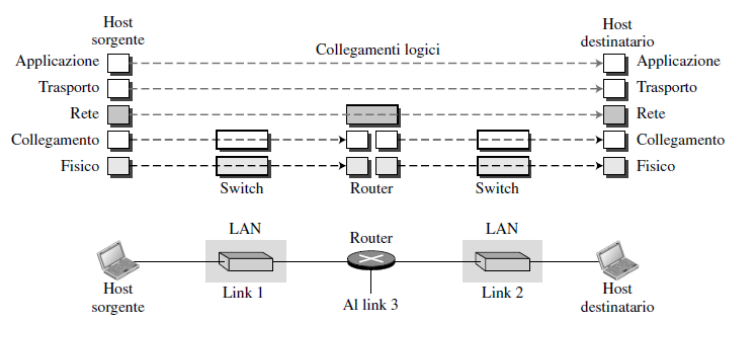
\includegraphics[width=10cm]{images/collegamento-logico2.PNG}
    \caption{Collegamenti logici fra i livelli dello stack protocollare TCP/IP}
    \label{fig:coll-livelli-tcp-ip}
\end{figure}

\subsection{Descrizione dei livelli dello stack protocollare TCP/IP}
Compreso il concetto di comunicazione logica, si descrivono brevemente i compiti di ciascun livello.

\subsubsection*{Livello applicazione}
Il collegamento logico fra i due livelli applicazione è end-to-end. I due livelli applicazione si scambiano dei messaggi come se fossero direttamente collegati. Naturalmente è necessario sapere che la comunicazione reale avviene attraversando tutti i livelli.

La comunicazione al livello applicazione avviene tra due processi (due programmi eseguiti a questo livello). Per comunicare, un processo invia una richiesta all'altro processo e ne riceve una risposta: la comunicazione processo-a-processo è il compito del livello applicazione.

I protocolli utilizzati in questo livello sono: HTTP (Hypertext Transfer Protocol), SMTP (Simple Mail Transfer Protocol), FTP (File Transfer Protocol), TELNET (Terminal Network), SSH (Secure Shell) e DNS (Domain Name System).

\subsubsection*{Livello trasporto}
Anche la connessione logica a livello di trasporto e end-to-end. Il livello di trasporto nell'host sorgente riceve il messaggio dal livello applicazione, lo incapsula in un pacchetto di livello di trasporto (chiamato segmento) e lo invia, tramite la connessione logica (virtuale), al livello di trasporto dell'host destinatario.

I protocolli principali in questo livello sono: TCP (Transmission Control Protocol) e UDP (User Datagram Protocol).

\subsubsection*{Livello rete}
Il compito del livello di rete (network) è quello di far arrivare i pacchetti dall'host sorgente all'host destinazione. La comunicazione a questo livello è host-to-host, ma dato che vi possono essere dei router nel tragitto fra la sorgente e la destinazione, questi hanno il compito di scegliere il miglior percorso (o rotta) per ciascun pacchetto. Si può affermare che il livello rete è responsabile della comunicazione host-to-host e dell'instradamento e inoltro dei pacchetti attraverso i possibili percorsi. 

Il livello rete in Internet comprende il protocollo principale, l'IP (Internet Protocol), che definisce il formato del pacchetto chiamato datagramma.

\subsubsection*{Livello di collegamento}
Si è visto come una internet sia costituita da più LAN e WAN interconnesse. Vi possono essere diversi percorsi (sequenze di link) anche parzialmente sovrapposti che un datagramma può utilizzare per viaggiare dalla sorgente alla destinazione. Quando un router ha determinato il link successivo da utilizzare, il livello di collegamento (data-link) si occupa di trasferire il pacchetto attraverso tale collegamento. E' anche possibile che vengano utilizzati protocolli differenti per ciascun tipo di link, in ogni caso il livello di collegamento si occupa del trasferimento del pacchetto attraverso il collegamento.

L'architettura TCP/IP non definisce alcun protocollo specifico per il livello di collegamento, ma supporta tutti i protocolli standard e proprietari. Qualsiasi protocollo che possa prendere in consegna il datagramma e trasferirlo attraverso il link è sufficiente per il livello rete. I pacchetti al livello di collegamento sono chiamati frame.

\subsubsection*{Livello fisico}
Il livello fisico si occupa di trasferire i singoli bit di un frame attraverso il link. Sebbene il livello fisico sia il livello più basso nella famiglia di protocolli TCP/IP, la comunicazione fra due dispositivi al livello fisico è ancora una comunicazione logica, poiché vi è un ulteriore livello nascosto: il mezzo trasmissivo al di sotto del livello fisico. Di conseguenza i bit ricevuti in un frame dal livello di collegamento vengono in realtà trasformati e inviati attraverso il mezzo trasmissivo, ma è comunque possibile pensare che l'unità logica trasmessa fra due livelli fisici in due dispositivi sia il bit.

\subsection{Incapsulamento e decapsulamento}
L'incapsulamento/decapsulamento è un concetto molto importante relativo alla strutturazione in livelli di una rete.

La Figura \ref{fig:incaps-decaps} illustra l'incapsulamento nell'host sorgente, il decapsulamento nell'host destinatario ed entrambe le operazioni nel router.

\begin{figure}[ht]
    \centering
    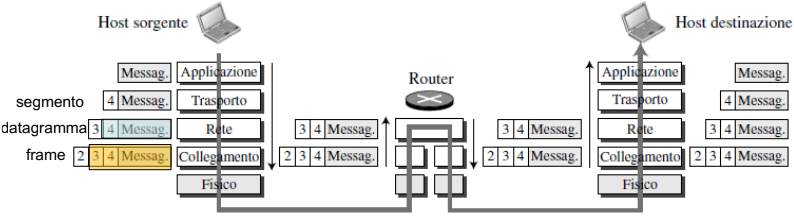
\includegraphics[width=12cm]{images/incaps-decaps.PNG}
    \caption{Incapsulamento e decapsulamento}
    \label{fig:incaps-decaps}
\end{figure}

La sorgente effettua esclusivamente l'incapsulamento.
\begin{enumerate}
    \item A livello applicazione i dati da scambiare vengono chiamati messaggi. Un messaggio solitamente non contiene alcuna intestazione (header) o trailer (informazioni di controllo in coda). Il messaggio viene passato al livello trasporto.
    \item Il livello trasporto considera il messaggio ricevuto come payload, ovvero come carico dati, che deve trasportare e gli aggiunge l'intestazione di livello trasporto che contiene varie informazioni per la gestione del pacchetto a quel livello (per esempio, gli identificatori dei programmi applicativi sorgente e destinatario, informazioni necessarie per la consegna end-to-end del messaggio ecc.). Questo procedimento di considerare il pacchetto ricevuto dal livello sovrastante come carico dati e aggiungergli un'intestazione è detto incapsulamento. Al livello di trasposto il risultato dell'incapsulamento è un segmento o un datagramma utente, a seconda del protocollo usato. Il livello trasporto passa quindi questo pacchetto al livello rete.
    \item Il livello rete considera il pacchetto di livello trasporto passatogli come proprio carico dati e gli aggiunge un'intestazione. Questo contiene gli indirizzi degli host sorgente e destinatario e altre informazioni utili. Il risultato è un pacchetto di livello rete, chiamato datagramma, che viene dunque passato al livello di collegamento.
    \item Il livello di collegamento considera il pacchetto di livello rete come payload e gli aggiunge la propria intestazione, che contiene l'indirizzo del livello di collegamento dell'host o del next-hop (il router). Il risultato è un pacchetto di livello di collegamento, chiamato frame, che viene quindi passato al livello fisico per la trasmissione.
\end{enumerate}

Nel router si effettua sia l'incapsulamento che il decapsulamento poiché questi è collegato a due o più link.
\begin{enumerate}
    \item L'insieme di bit ricevuti dal livello fisico viene passato al livello di collegamento, che decapsula il frame (ovvero rimuove l'header) e passa il datagramma al livello di rete.
    \item Il livello di rete consulta solamente gli indirizzi di sorgente e destinatario nell'header del datagramma e consulta la propria tabella di instradamento per decidere il next-hop al quale consegnare il datagramma. Il datagramma viene quindi passato al livello di collegamento del link interessato.
    \item Il livello di collegamento incapsula quindi il datagramma in un frame e lo passa al livello fisico per la trasmissione.
\end{enumerate}

Ciascun livello nell'host destinatario rimuove la propria intestazione dal pacchetto ricevuto estraendone il payload; questo viene passato al protocollo del livello sovrastante, fino a quando il messaggio raggiunge il livello applicazione.

\subsection{Indirizzamento}
E' necessario presentare un altro concetto relativo alla gerarchia di livelli in Internet: l'indirizzamento. Come discusso in precedenza, questo modello prevede una comunicazione logica fra coppie di livelli. Qualsiasi comunicazione che coinvolge due parti richiede due indirizzi: l'indirizzo sorgente e l'indirizzo destinazione. Sebbene possa sembrare che siano necessarie cinque paia di indirizzi, un paio per livello, normalmente è sufficiente utilizzarne solo quattro poiché il livello fisico non richiede indirizzi: l'unità dati scambiata a livello fisico è infatti il bit, che decisamente non può avere un indirizzo. 

\begin{figure}[ht]
    \centering
    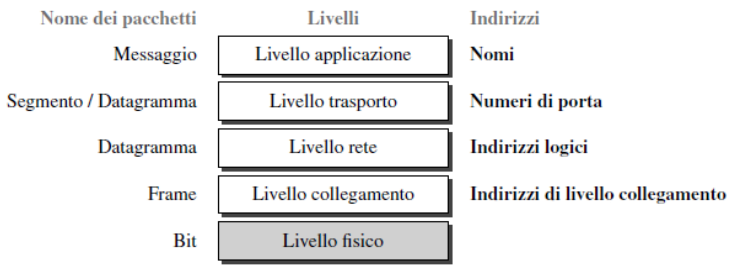
\includegraphics[width=10cm]{images/indirizzamento.PNG}
    \caption{Indirizzamento nel modello TCP/IP}
    \label{fig:indirizzamento-tcp-ip}
\end{figure}

Come evidenziato in Figura \ref{fig:indirizzamento-tcp-ip} esiste una relazione fra livello, indirizzo utilizzato in quel livello e nome del relativo pacchetto.

\subsection{Multiplexing e demultiplexing}
Dato che lo stack protocollare TCP/IP prevede più protocolli nello stesso livello, è necessario eseguire il multiplexing alla sorgente e il demultiplexing alla destinazione. Multiplexing in questo caso significa che un protocollo di un livello può incapsulare (uno alla volta) i pacchetti ottenuti da più protocolli del livello immediatamente superiore; demultiplexing significa che un protocollo può decaspulare e consegnare i pacchetti a più protocolli del livello immediatamente superiore.

\begin{figure}[ht]
    \centering
    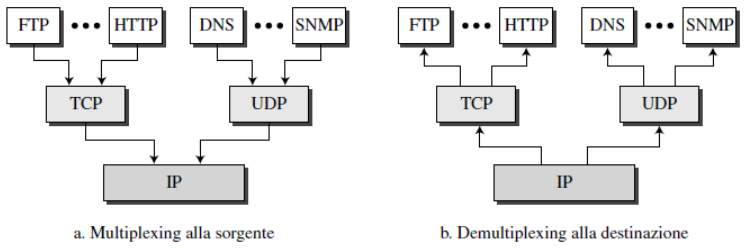
\includegraphics[width=10cm]{images/multiplexing-demultiplexing.PNG}
    \caption{Multiplexing e demultiplexing}
    \label{fig:multiplexing-demultiplexing}
\end{figure}

Per poter effettuare le operazioni di multiplexing e demultiplexing un protocollo deve avere un campo nel proprio header per identificare a quale protocollo appartengano i pacchetti incapsulati.

\section{Il modello OSI}
Sebbene nel contesto di Internet il modello TCP/IP sia quello più diffuso, esso non è l'unico modello esistente. L'ISO (International Organization for Standardization), fondata nel 1947, è un'organizzazione internazionale dedicata alla definizione di standard universalmente accettati, organizzazione di cui fanno parte oltre tre quarti delle nazioni. Il modello OSI (Open Systems Interconnection) è uno standard ISO, introdotto alla fine degli anni '70, che concerne tutti gli aspetti della reti.

Un sistema aperto è un insieme di protocolli che consente a due sistemi qualsiasi di comunicare indipendentemente dalla loro (differente) architettura sottostante. Lo scopo del modello OSI è facilitare la comunicazione fra sistemi di comunicazione differenti senza dovere imporre vincoli alla logica dell'hardware e del software utilizzati. Il modello OSI non è un protocollo, ma un modello per comprendere e progettare architetture di rete flessibili, robuste e interoperabili. E' stato dunque ideato come base per lo sviluppo di protocolli dello stack OSI.

Il modello OSI è un framework stratificato per il progetto di sistemi di rete che consentono la comunicazione fra qualsiasi tipo di dispositivo. E' suddiviso in sette livelli ognuno dei quali descrive una parte del meccanismo di trasferimento dell'informazione attraverso una rete.

Confrontando il modello OSI con il modello TCP/IP si scopre che nell'architettura TCP/ IP mancano i livelli sessione e presentazione. Questi due livelli vengono solitamente considerati parte del livello applicazione di TCP/IP.

\begin{figure}[ht]
    \centering
    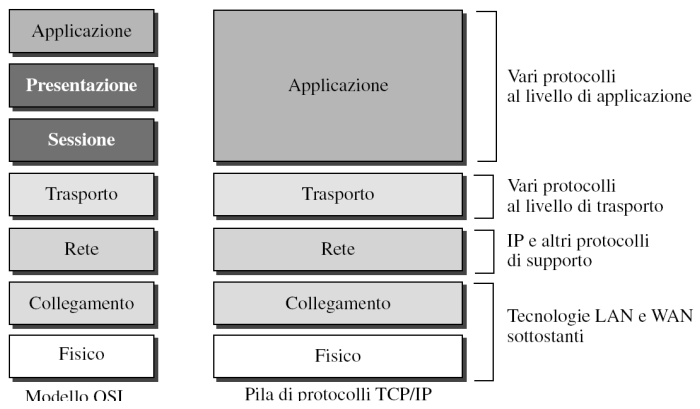
\includegraphics[width=9cm]{images/OSI.PNG}
    \caption{TCP/IP e il modello OSI}
    \label{fig:OSI}
\end{figure}

\subsection{L'insuccesso del modello OSI}
Il modello OSI venne pubblicato dopo la definizione dell'architettura TCP/IP e la maggior parte degli esperti arrivò a ipotizzare che avrebbe completamente rimpiazzato TCP/IP. In realtà questo non avvenne per varie ragioni. Per prima cosa l'OSI venne pubblicato quando il TCP/IP era già ampiamente diffuso e gli si erano già dedicate notevoli risorse: un'eventuale sostituzione avrebbe rappresentato un costo notevole. La seconda ragione è che alcuni livelli nel modello OSI, come presentazione e sessione, non sono mai stati completamente specificati: il software corrispondente non è dunque mai stato completamente sviluppato. Infine anche quando alcune organizzazioni implementarono l'OSI in qualche applicazione, non riuscirono a dimostrare delle prestazioni tali da convincere le autorità di Internet a sostituire il TCP/IP con il modello OSI.